\documentclass[11pt,a4paper]{article}

\usepackage[utf8]{inputenc}
\usepackage[T1]{fontenc}
\usepackage[english]{babel}
\usepackage{verbatim}
\usepackage{amsfonts}
\usepackage{amssymb}

\usepackage{amsmath}
\DeclareMathOperator*{\argmax}{argmax}
\DeclareMathOperator*{\argmin}{argmin}
\DeclareMathOperator*{\med}{med}

\usepackage{amsthm}
\usepackage{graphicx}
\usepackage{lmodern}
\usepackage{empheq}
\usepackage{epsfig}
\usepackage{tikz}
\usepackage{xcolor}
\usepackage{algorithm}
\usepackage{algorithmic}
\usepackage{fancyvrb}
\usepackage{moreverb}
\usepackage{listings}
\usepackage{url}
%%\usepackage[round]{natbib}

\setlength{\unitlength}{1mm}
\usepackage{pstricks}

\usepackage[top=3cm, bottom=3cm, left=3cm, right=3cm]{geometry}

%%\usepackage{hyperref}

\begin{document}
\section{Introduction}
While many algorithm for learning from demonstration are based on training data, we propose to leverage the interaction between the teacher and learner. We believe that learning from demonstration with natural interaction has many advantages. It allows easy reprogramming of the robot since data acquisition in laboratory framework is not necessary. Moreover, the robot can interrupt the demonstration and engage in an interaction with the teacher in order to disambiguate its understanding, reducing the amount of data needed for learning.
\newline
In order to allow natural interaction, we rely on non-intrusive recording systems. Teaching from demonstration involves many communication cues. The language informed about the objects and the task to perform nevertheless other non-verbal communication cues carry those informations too. In particular, the gaze is an important one. 
\newline
The gaze informs about attention and intention. Therefore, it can be used as a prior for task segmentation and recognition. The estimation of the gaze relies on the algorithm presented in \cite{Funes2016} where the gaze is infrared from RGB and Depth video steams obtained from a Microsoft Kinect.

\section{Motivation}
The present dataset is used to evaluate the gaze estimation algorithm. As a first step, we aim to evaluate the accuracy of the gaze estimation algorithm using a controlled (supervised) calibration procedure. Furthermore, we will use the human-robot interactions to define an unsupervised calibration method. In particular, we are interested in calibration methods using interaction cues to infer targets of calibration. As a second step, we aim to leverage gaze behavior during demonstration. In particular, the segmentation and recognition of the demonstration.
\subsection{Gaze calibration}
\paragraph{Supervised}: The gaze calibration procedure relies on the definition of targets for calibration. In the case of point (marker) targets, the target is trivially defined. The present data set aims to provide enough calibration points to evaluate the gaze estimation algorithm with a calibration procedure. Nevertheless, the inference of the gaze target is less trivial when the object of attention is big with respect to some dimensions. We will be interesting to evaluate the effect of the gaze calibration procedure while the target is an object (of various size and shape).
\paragraph{Unsupervised}: Interaction cues can be used for the definition of targets for calibration. In \cite{Siegfried2017}, the authors rely on the conversational interaction between the people; we look at the person we talk to. While performing object related actions, the gaze fixation at the object usually precedes the grasping of the object and the fixation at the landing position precede the placing \cite{Land2009} (and more).

\subsection{Gaze behavior}
Based on the accuracy of the gaze estimation algorithm, we would like to leverage some gaze behaviors. In particular, we evaluate how well the gaze estimation algorithm can inferred the Visual Focus Of Attention (VFOA). Further, we would like to incorporate the VFOA model in a multi-modal task segmentation and recognition methods. In particular, we are interesting in the classification of the VFOA as reactive and proactive in order to segment and recognize demonstrations.

\section{Data collection}
\label{Data_Collection}
In this section, we first describe our recording methodology and then describe the different recording sessions constituting the dataset.
\subsection{Overview}
\label{Overview}
\begin{figure}[!ht]
\begin{center}
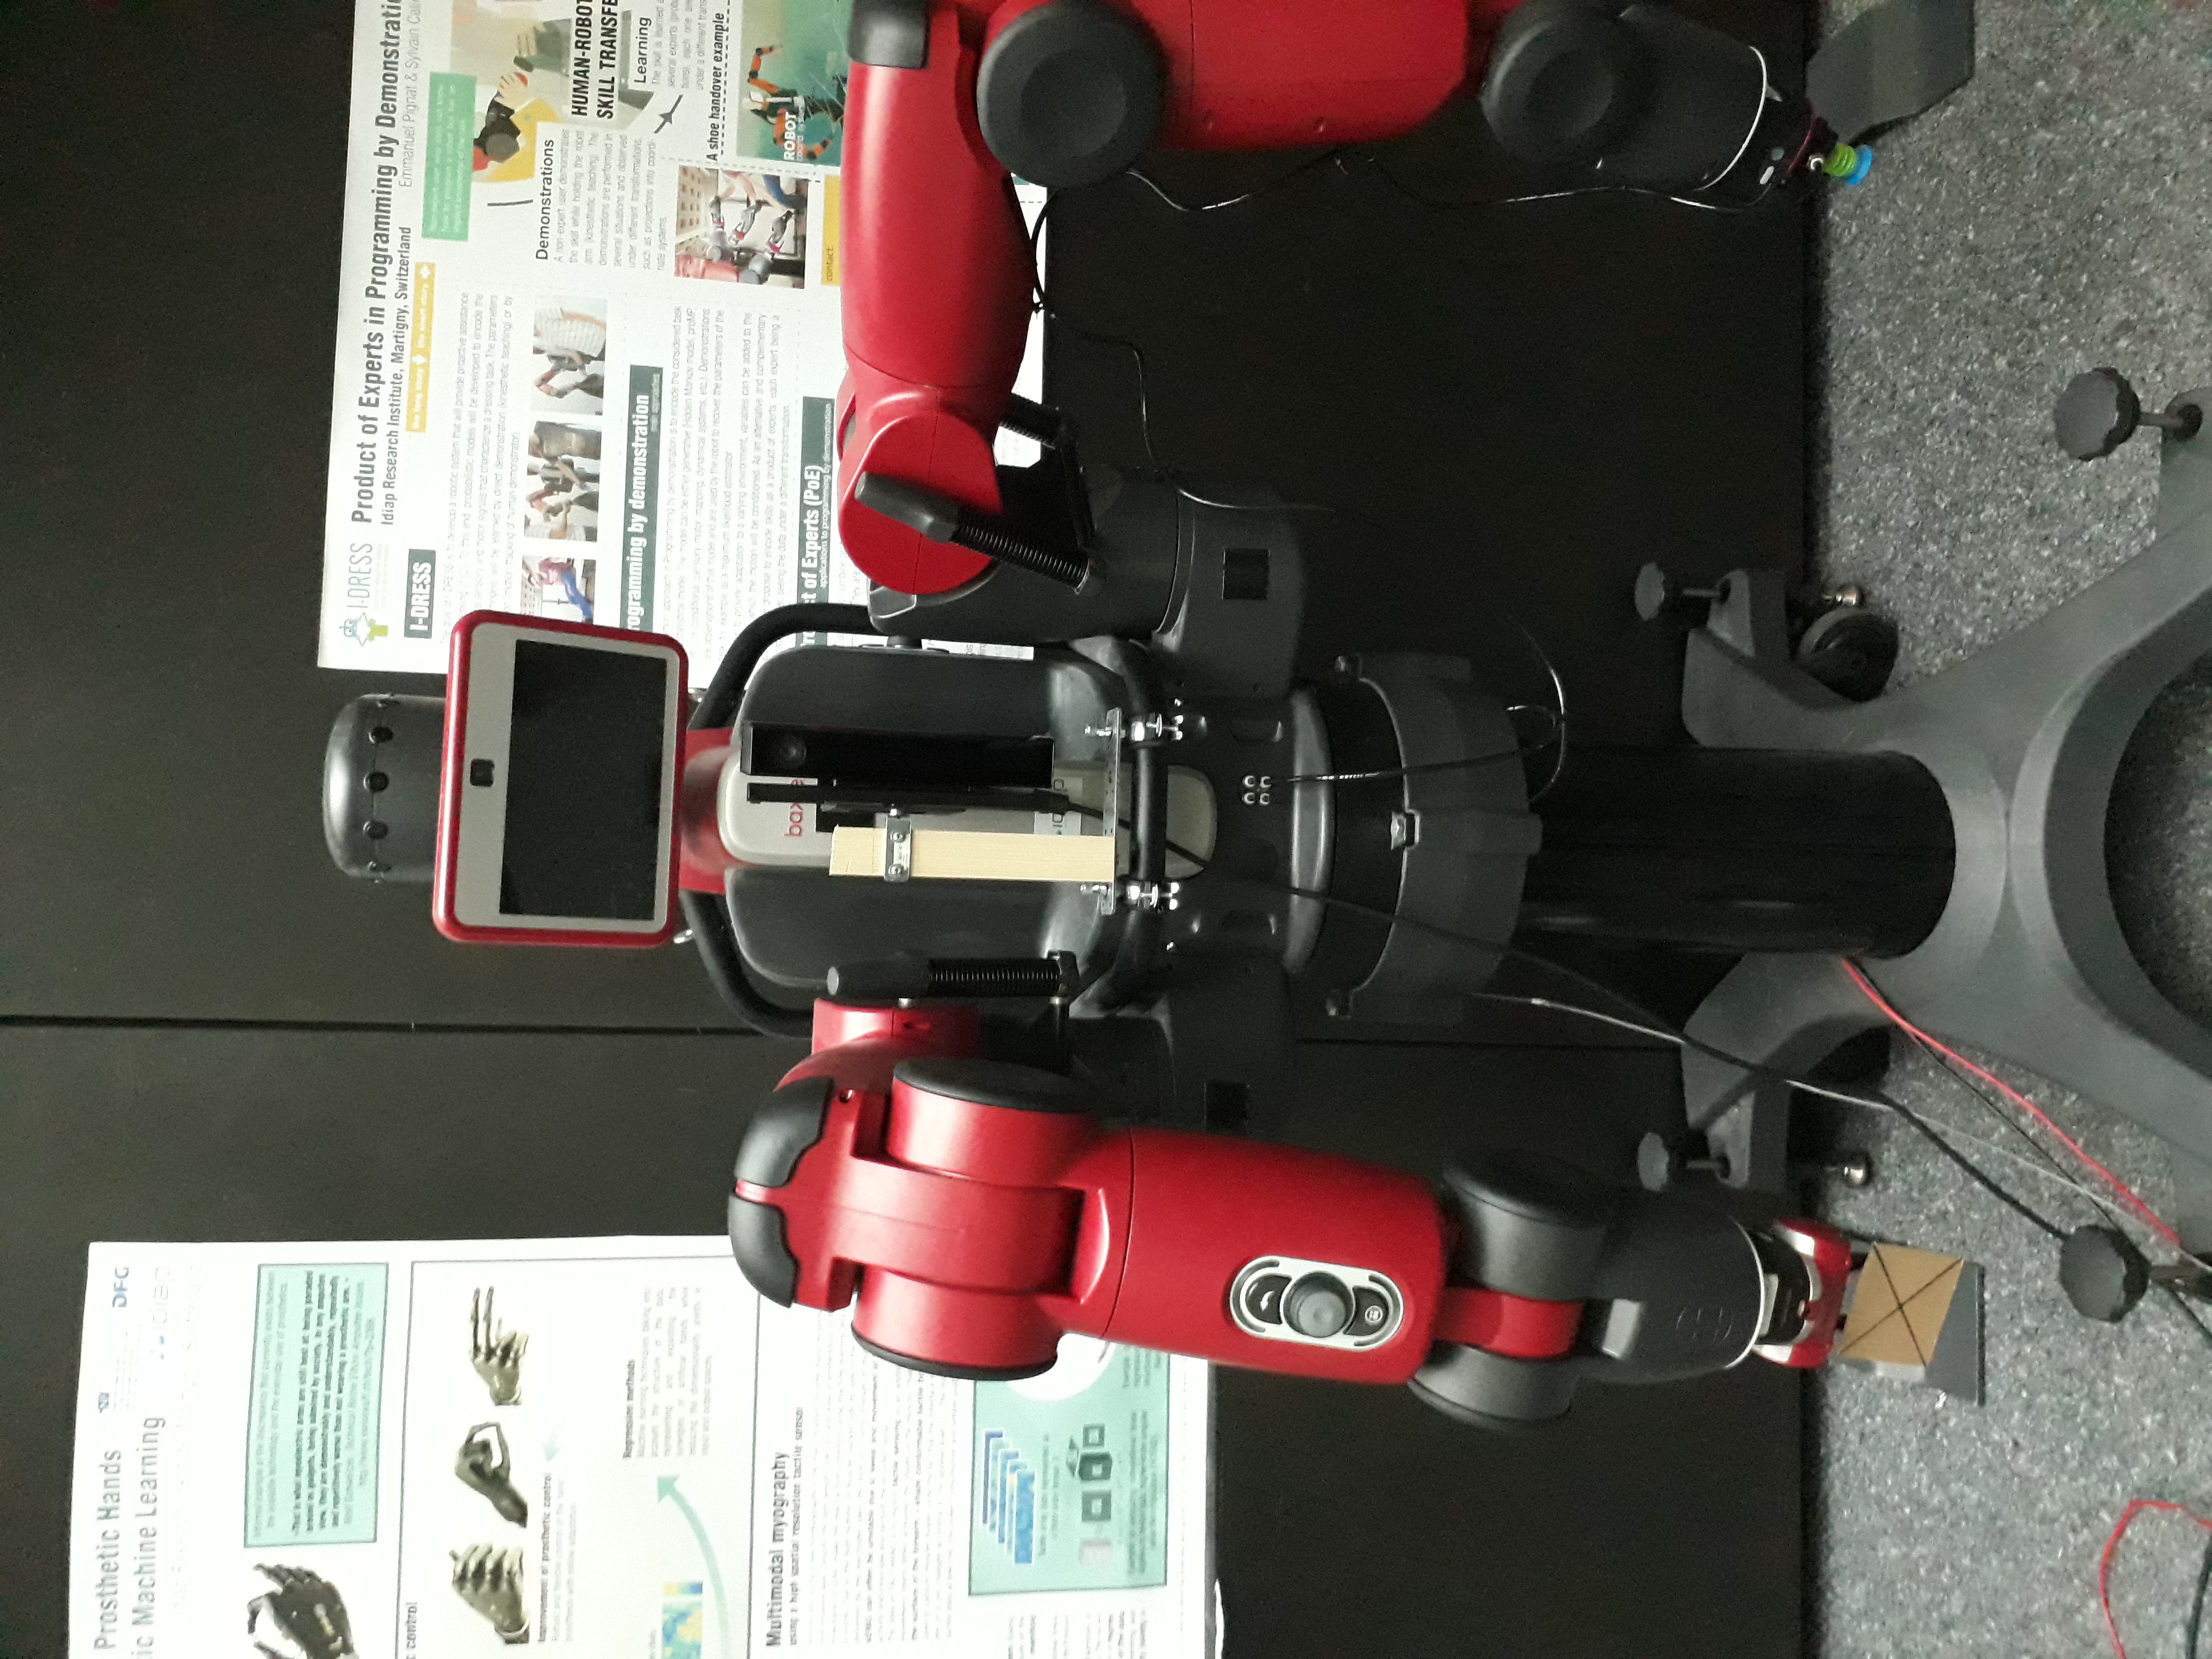
\includegraphics[scale=0.05, angle=-90]{Pictures/Baxter_Setup.jpg}
\end{center}
\caption{Experimental setup. \label{Experimental_Setup}}
\end{figure}
The recording setup is as shown in figure \ref{Experimental_Setup}. It comprises a RGB-D camera (a Microsoft Kinect v2), a robot (a Baxter from Rethink Robotics), a table with marker, a cup, a saucer,.... The characteristics and purpose or function of each element are as follow:
\begin{itemize}
\item Microsoft Kinect v2: this consumer device provides standard video (RGB) and Depth video steams. The RGB camera has an HD resolution ($1920 \times 1080$) while the Depth camera has a resolution of $512 \times 424$. The acquisition rate is 30 frame-per-second.
\item Baxter robot: this is a human like robot from Rethink Robotics. We will use the robot's ego-motion to infer gaze target. In particular, the position of the head of the robot (screen) and its end-effectors are recored.
\item Table with markers: those markers are used as calibration targets for the gaze. Moreover, the object are placed on those markers in order to infer qualitatively there position without the need of an object detection algorithm. The markers are numbered in order to differentiate them.
\item Objects: it comprises: a cup, a saucer, a knife, a fork, a dish, a glass and a marble. Those objects are used as gaze target for calibration. Moreover, those objects are common in everyday life routines and will be used for the task of setting a table. We provide a 3D mesh for each objects.
\end{itemize}

The calibration and synchronization of the robot and the camera are explained session~\ref{Data_Collection}.

\subsection{Recording sessions}
In the following sections, the various experiments are described and motivated.
\subsubsection{Static-pose and end-effector target (SP-ET)}
The end-effector of the robot is used as a target for calibration. More precisely, A white rubber band is scotched to each gripper of the robot as shown on figure XXX. The participant is asked to look at the camera (kinect) on the chest of the robot in order to guarantee, more or less, a frontal image of the face. Once the participant is ready, it will be asked to keep his head pose fixed during the calibration procedure. The latter consists in ...
\paragraph{Motivation}
The algorithm for gaze estimation is based on the evaluation of the head pose. Indeed, based on the head position and orientation, a frontal image of the face is computed. In order to avoid errors of the gaze estimation due to the frontalization procedure, a static head pose is imposed. We are interested in the evaluation of the gaze estimation algorithm independently of the frontalization procedure. In particular, how calibration is affected. (need clarification)

\subsubsection{Natural-pose and end-effector target (NP-ET)}
The end-effector of the robot is used as a target for calibration as described in the precedent recording session (SP-ET). In the present recording session, the participant is free to move his head. The calibration procedure consists in ...
\paragraph{Motivation}
We are interested of testing our calibration algorithm in a more natural setup. In particular, we want to evaluate our gaze estimation algorithm with respect to the head pose and how the latter affects the calibration procedure. Moreover, the calibration of the gaze tracker using the SP-ET and NP-ET recording sessions will be used to evaluate our unsupervised calibration method based on interactions.

\subsubsection{Markers on the table targets (MT)}
In this recording session, the numbered markers on the table are used as targets for calibration (see figure XXX). The participant starts by looking at the robot face (screen). The robot asks: 
\begin{center}
"\textit{Can you see the marker number \texttt{XXX}?}" 
\end{center}
And wait for the response. Then it asks: 
\begin{center}
\textit{Can you show it to me, please?}"
\end{center}
The robots repeat the questions for ten different marker numbers chosen randomly. The supervisor of the recording session will handle the timing of the utterance on-line.
\paragraph{Motivation.}
The MT recording session provides additional points for calibration with natural head pose. In particular, the calibration points are contains in the working region for the future recording sessions. Beside, the supervised calibration of our gaze tracker, we are interested in the gaze behavior during interaction. The MT recording provides two types of interaction. The first question may produce a gaze at the marker. The interaction can be split in 4 steps: listen, search, find, answer. That will be interested to segment and recognize for our future research. The second question produce another type of interaction involving pointing gesture. We believe that gaze and pointing  are strongly coordinated and may give a strong prior for an unsupervised calibration the gaze estimation algorithm.
 
\subsubsection{Object on the table target (OT)}
We will provide 10 different setups involving five objects (marble, knife, glass, dish, cup) randomly placed on the marker of the table. The participant is facing the robot, waiting for interaction. The robot asks: 
\begin{center}
"\textit{Where is the \texttt{<object>}?}"
\end{center}
And wait for an answer. The robot asks the question for all the five objects. For each participant, we will choose randomly two out of the ten different setups
\paragraph{Motivation.} 
The present recording session is quiet similar to the MT recoding. Nevertheless, it differs with respect to two aspects. First, the points of fixation are not as trivial as in the case of markers on the table. The marble is a small object similar to the markers. The knife is long object. The glass is a vertical object. The dish is a large object and the cup is a non-symmetrical middle size object. In particular, we are interested in the effect of different sizes and shapes of objects on the calibration of the gaze estimation algorithm. Moreover, the OT recording provides a slightly different interaction. The participants are more free to choose there way of explaining "\textit{where is the \texttt{<object>}}". Some participants may prefer to point to the object or only look at the object. While some others will refer to the position of the object with respect to the table or the other objects on the table. This aspect of interaction will be interested for our future research. 


\subsubsection{Put on, then move on (Pon-Mon)}
We will provide 20 different setup involving three objects chosen randomly from the seven objects (see section \ref{Overview}) and placed randomly on the markers. Depending on the chosen objects, the participant is asked to execute the following task:
\begin{center}
\textit{Put the \texttt{<object1>} on the \texttt{<object2>}. Then, move the \texttt{<object2>} (with \texttt{<object1>} remaining on) on marker number \texttt{XXX}.}
\end{center}
For each participant, we will choose randomly five out of the twenty different setups.
\paragraph{Motiviation.} Through this recording session, we aim to use interaction cues for an unsupervised calibration procedure. The demonstration consists in two pick an place. Using gaze prior as given in \cite{Land2009}, we aim to test our calibration procedure. Moreover, we are interested in task segmentation and recognition. In particular, we want to know if the gaze estimation algorithm can capture a difference in the gaze behavior between the two pick-and-place demonstrations. Moreover, we will experiment different size and shape of objects and initial position (distance between the objects may influence the calibration procedure).

\subsubsection{Put on, then move on, interaction (Pon-Mon-Int)}
The present experiment is similar to the previous one (Pon-Mon), except that it will be asked to the participant to explain what they do to the robot during the manipulation.
\paragraph{Motivation.}
We believe that human behaviors change when we explain what we are doing (legible motion). The present experiment will provide data for learning a task from demonstration based on interaction (the participant explaining to the robot).

\subsubsection{Put on, then throw in (Pon-Tin)}
We will provide 20 different setup involving a marble and three objects chosen randomly from the seven objects (see section \ref{Overview}) and placed randomly on the markers. Depending on the chosen objects, the participant is asked to execute the following task:
\begin{center}
\textit{Put the marble on/in \texttt{<object1>}. Then, throw the marble (without touching it, that is, using only the \texttt{<object1>}) in the \texttt{<object2>}}
\end{center}
For each participant, we will choose randomly five out of the twenty different setups.
\paragraph{Motivation.} The present recording session is slightly similar to the Pon-Mon recording. Nevertheless, in the Pon-Tin recording session the first object is always the marble. The latter is a clear point and the potential region of attention can be defined accurately. The second step of the recording session involves a different dynamic than the Pon-Mon recording (develop more). In particular, we want to know if the gaze estimation algorithm can capture any difference in gaze behavior between the different object involved, as well as, between the Pon-Mon recording.

\subsubsection{Put on, then throw in, interaction (Pon-Tin-Int)}
The present experiment is similar to the previous one (Pon-Tin), except that it will be asked to the participant to explain what they do to the robot during the manipulation.
\paragraph{Motivation.}
We believe that human behavior change when it explains what s/he is doing (legible motion). The present experiment will provide data for learning a task from demonstration based on interaction (the participant explaining to the robot).

\subsubsection{Set a table (ST)}
We will provide 10 different setup involving a knife, a fork, a dish and a glass placed randomly on the markers. The participant is asked to set a table (fork, knife, spoon, dish, glass). It will be asked to the participants to explain what they do to the robot when performing the task. We will randomly choose five out of the ten different setups for recording.
\paragraph{Motivation.}
The present recording session involves a more natural demonstration of a task. The number of object involved in the interaction are higher than the previous recording sessions. Moreover, the task is segmented in more subtask. We are interested to know if we can calibrate our gaze estimation algorithm through this interaction, as well as, segmented and recognition of the task presented.



\section{Data processing}
\label{Data_Processing}
Besides the raw data describe in section \ref{Overview}, we also provide additional information that is essential for deriving ground truth measures for evaluation or simply useful to exploit the dataset and run the experiments. It compromises the camera calibration, the synchronization, the head pose, the manual annotations, the target position, and 3D object meshes. Below, we present the procedure to estimate those parameters

\subsection{World coordinate system definition}
To standardize the definition all 3D variable in the data, we have defined a common world coordinate system (WCS), in which the variable refers to \textit{meters}. It has been define as the robot frame being at the base of the robot.

\subsection{RGB-D sensors intrinsic calibration}
For the calibration of the Microsoft Kinect v2, we rely on the \texttt{iai\_kinect} softwares. It computes the intrinsic of the RGB and Depth camera, as well as the extrinsic parameters between both cameras.

\subsection{RGB-D sensors extrinsic calibration and synchrony}
The rigid transform from the robot to the camera frame can be evaluated using the position of the end-effector in the RGB-D camera. The synchronization of the robot and camera use done by time-stamping the robot time with the computer and using the \texttt{MessageFilter} ROS package.

\subsection{Target position}
By placing the object on the markers of the table, one can evaluate there position when there are on the table. In the future, we will provide object position using our 3D meshes of the object or an other methods based on object detection. Nevertheless, we have to provide a ground truth for the gaze during OT (in particular). We ask to the participants which part of the object they look at. We report those region on pictures of the object. The position of the target is given for each frame. Each object has its own ID which is given in the data set. Moreover, an additional variable is set to "left", "right" or "NA" if the object is manipulated, respectively, by the left, the right hand or is not manipulated.

\subsection{Body landmark}
We will report body landmark position as hands, shoulders and head pose using our tracker (REFERENCE).

\subsection{Gaze behavior label}
Each frame is labeled with a "b" when the participant is blinking. The frame is labeled by the object ID when the participant is looking at the object. In the case of saccade or undefined VFOA (gaze search), the frame is labeled with "NA". This labeling is done manually. 
\paragraph{Remark}
For the RT recording, the target is not visible in the RGB stream. Therefore, it is difficult to label the gaze at the end-effector. One could to the labeling during the recording when the supervisor has a complete view of the scene. Another possibility consists in recording again if the participant has been distracted. The check is done during the recording.

\section{Unsupervised gaze calibration}
\begin{figure}[!ht]
\begin{center}
\includegraphics[scale=0.5]{Pictures/GazeObjectBehavior_Land.png}
\end{center}
\caption{Results from \cite{Land2009}. (\textbf{A}) The relative timings of body movements, fixations on particular objects, and manipulation of those objects by the hands during the first 70 s of a tea-making session.
(\textbf{B}) Average relative timings of trunk movements,
fixations on particular objects (which may involve several individual fixations), and manipulation of those objects. The data represent
94 object-related actions from three subjects. Typical actions last about 3 s (extended waiting periods, such as watching for the kettle to
boil, have been excluded). Note that trunk movements (when present) precede fixations, which precede manipulation, by about 0.6 s in
each case. Similarly, fixation moves on to the next object about 0.6 s before manipulation is complete. There are wide variations in timing
(histograms), with manipulation sometimes preceding gaze fixation.\label{LandResults}}
\end{figure}


\clearpage
\bibliographystyle{ieeetr}
\bibliography{Notes}

\end{document}